\documentclass[9pt, mathserif, aspectratio=43]{beamer}

\usepackage{AcademicSlides}
% \usepackage{ctex}
\usepackage{media9}
\usepackage{ragged2e}
\usepackage{sidecap}
\makeatletter
\def\blfootnote{\gdef\@thefnmark{}\@footnotetext}
\makeatother
\sidecaptionvpos{figure}{c}

\setbeamertemplate{caption}[numbered]


\renewcommand*{\thefootnote}{\fnsymbol{footnote}}


% \usetheme{Warsaw}
\usetheme{Madrid}

% \usefonttheme{serif}
% \usefonttheme{professionalfonts}
% \usepackage{arev}
% \setbeamertemplate{footline}{%
   % \raisebox{5pt}{\makebox[\paperwidth]{\hfill\makebox[10pt]{\scriptsize\insertframenumber}}}}
\useoutertheme{default}
% \useoutertheme{infolines}
\setbeamertemplate{footline}
{
  \leavevmode%
  \hbox{%
  \begin{beamercolorbox}[wd=.2\paperwidth,ht=2.25ex,dp=1ex,center]{author in head/foot}%
	\usebeamerfont{author in head/foot}\insertshortauthor\ (\insertshortinstitute)
  \end{beamercolorbox}%
  \begin{beamercolorbox}[wd=.5\paperwidth,ht=2.25ex,dp=1ex,center]{title in head/foot}%
      \usebeamerfont{title in head/foot}{\insertshorttitle}
  \end{beamercolorbox}%
  % \begin{beamercolorbox}[wd=.333333\paperwidth,ht=2.25ex,dp=1ex,right]{date in head/foot}%
	% \usebeamerfont{date in head/foot}\insertshortdate{}\hspace*{2em}
	% \insertframenumber{} / \inserttotalframenumber\hspace*{2ex} 
  % \end{beamercolorbox}}%
  % \begin{beamercolorbox}[wd=.25\paperwidth,ht=2.25ex,dp=1ex,right]{date in head/foot}%
	% \usebeamerfont{date in head/foot}\insertshortdate{}\hspace*{2em} Page
	% \insertframenumber{} \hspace*{2ex} 
  % \end{beamercolorbox}}%
  \begin{beamercolorbox}[wd=.3\paperwidth,ht=2.25ex,dp=1ex,right]{date in head/foot}%
	\usebeamerfont{title in head/foot}\insertshortdate{}\hspace*{1em} Page
	\insertframenumber{} \hspace*{2ex} 
  \end{beamercolorbox}}%
  \vskip0pt%
}
\hypersetup{colorlinks=false}


% \titlegraphic{\includegraphics[width=1.6cm]{img/njulogoaipurple.eps}\hspace*{.75cm}~%
   % \includegraphics[width=1.6cm]{img/logoia.jpg}
% }
\titlegraphic{
    % 
\includegraphics[height=1.5cm]{fig/NJU_logo.jpg}
    % \\[0.3cm]
    % \hspace{1cm}
    % 
\includegraphics[height=1.5cm]{fig/UTS_logo.jpg}
    % \qquad
    
\includegraphics[height=1.5cm]{fig/PSU_logo.png}
}


\let\emph\relax % there's no \RedeclareTextFontCommand
% \DeclareTextFontCommand{\emph}{\bfseries\em}
% \DeclareTextFontCommand{\emph}{\bfseries}
\DeclareTextFontCommand{\emph}{\bfseries\sffamily}

\author[\textsc{Jiaxin Zhong}]{\textsc{\underline{Jiaxin Zhong}} }
\institute[PSU]{\large The Sound Innovation of Metamaterials and Biomedical Acoustics (SIMBA)\\ The Pennsylvania State University (PSU)}
\date{\today}
\title[Short Title]{{\huge Main Title} \\[0.3cm] Here Goes the Subtitle}


\setbeamerfont{footnote}{size=\scriptsize}
\usepackage{caption}
\captionsetup{font = scriptsize, labelfont = scriptsize}

%% reference
\bibliography{ref}

% \usepackage{mlmodern}
\begin{document}

\maketitle
\begin{frame}{Outline}
    \begin{itemize}
        \LARGE 
    \item Introduction
    \item Main section 1
    \item Main section 2
    \item Conclusions and future work
    \end{itemize}
\end{frame}

\begin{frame}{Introduction}
    This is a template for the academic presentation.
    \begin{block}{Block title}
        \begin{itemize}
            \item Line 1
            \item Line 2
        \end{itemize}
    \end{block}
    \begin{exampleblock}{Example block title}
        Description here
        \begin{itemize}
            \item Line 1
            \item Line 2
        \end{itemize}
    \end{exampleblock}
\end{frame}

\begin{frame}
    \frametitle{Sample slide --- Research experience: PhD work}
    Sound fields on \emph{front side}:
    \begin{itemize}
        \item \emph{Near field}: second-order nonlinear or Kuznetsov equation (local effects are strong)
    \item \emph{Westervelt far field}: Westervelt equation (local effects are negligible)
    \item \emph{Inverse-law far field}: $p \propto 1/r$
            % \2 $R_1$: \emph{transition distance} from near field to Westervelt far field (0.1 m)
            % \2 $R_2$: \emph{transition distance} from Westervelt far field to inverse-law far field (30 m)
        % \1 Back side
        \item Proposed simple formulae for the \emph{transition distances}
        \end{itemize}
    \begin{columns}
        \column{0.4\textwidth}
        \begin{figure}[!htb]
        \centering
        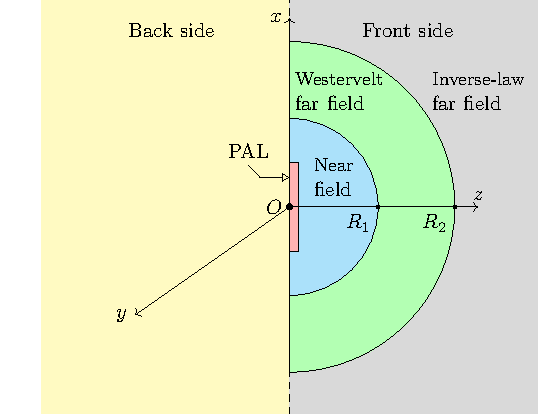
\includegraphics[width = \textwidth]{fig/pal_sound_field_220117A.pdf}
        \caption{Sound fields generated by a PAL.}
    \end{figure}
    \column{0.55\textwidth}
    \begin{figure}[!htb]
        \centering
        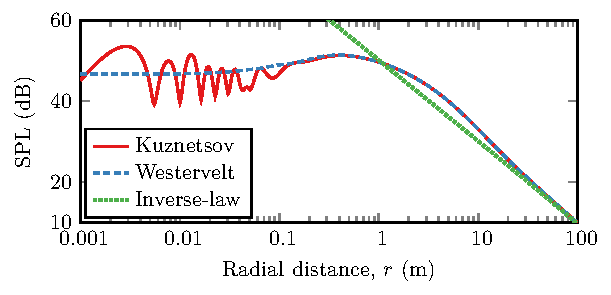
\includegraphics[width = \textwidth]{fig/fullfield_a0p05_ultra40e3_audio1000_angle0_200802H_v2.pdf}
        \caption{Audio SPL as a function of the propagating distance at 1 kHz.}
    \end{figure}
    \end{columns}
    \blfootnote{
        References:
        \begin{enumerate}
            \item \fullcite{Wen1988DiffractionBeamField}
        \end{enumerate}
        }
\end{frame}

\begin{frame}
    \frametitle{Sample slide --- Research experience: PhD work}
    Sound fields on \emph{back side}:
    \begin{itemize}
        \item Proposed a \emph{non-paraxial theoretical model} validated by experiments
    \item Audible sound behind a PAL especially at \emph{low frequencies} 
    \end{itemize}
\begin{figure}[!htb]
    \centering
    \begin{columns}
        \column{0.4\textwidth}
    \begin{subfigure}{\textwidth}
        \centering
        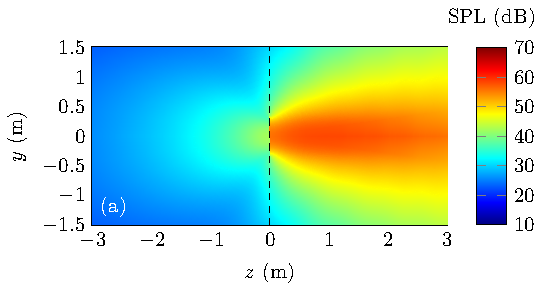
\includegraphics[width = \textwidth]{fig/ComparePalAudio2D_Simulation_315Hz.pdf}
    \end{subfigure}
    \\[-.3cm]
    \begin{subfigure}{\textwidth}
        \centering
        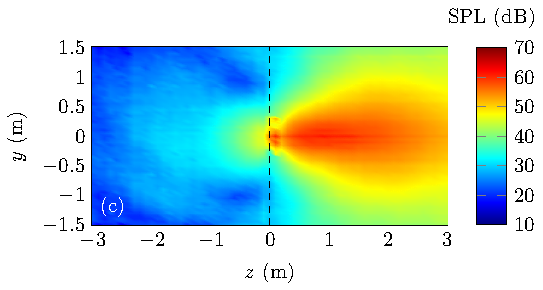
\includegraphics[width = \textwidth]{fig/ComparePalAudio2D_Experiment_315Hz.pdf}
    \end{subfigure}

    \column{.4\textwidth}
    \begin{subfigure}{\textwidth}
        \centering
        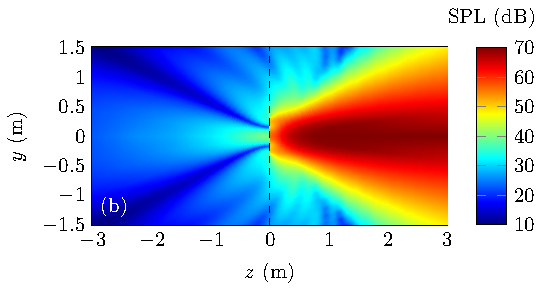
\includegraphics[width = \textwidth]{fig/ComparePalAudio2D_Simulation_800Hz.pdf}
    \end{subfigure}
    \\[-.3cm]
    \begin{subfigure}{\textwidth}
        \centering
        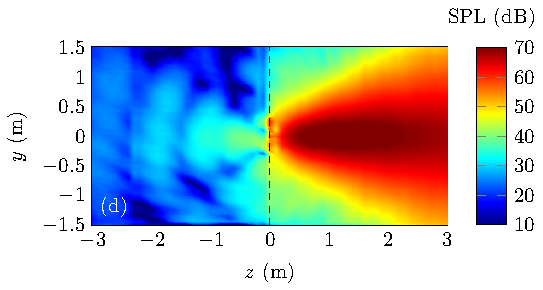
\includegraphics[width = \textwidth]{fig/ComparePalAudio2D_Experiment_800Hz.pdf}
    \end{subfigure}
    \column{.2\textwidth}
    \caption{Audio SPL. Left column, 315 Hz; right column, 800 Hz; top row, simulations; bottom row, measurements.} 
    \end{columns}
\end{figure}
    \blfootnote{
        References:
        \begin{itemize}
            \item \fullcite{Wen1988DiffractionBeamField}
        \end{itemize}
        }
\end{frame}

\begin{frame}{Sample slide --- Research experience: PhD work}
    \emph{Improved numerical methods} 
    \begin{itemize}
        \item Difficulty: nonlinear wave equation
        \item Proposed a \emph{spherical wave expansion} based on both \emph{Westervelt} and \emph{Kuznetsov} equations
        \item $100\sim 500$ times faster than the existing method
        \item Without loss of accuracy
        \item Fast and reliable simulations in ANC and other audio applications
\end{itemize}
    \begin{equation}
        \text{Existing method:}
        \qquad p(\vb{r}) = \iiiiint 
        \cdots
        \dd^2 \vb{r}' \dd^3 \vb{r}''
    \end{equation}
    \begin{equation}
        \text{Proposed method:}
        \qquad p(\vb{r}) = \sum\sum\sum\sum \int 
        \cdots \dd r'
    \end{equation}
    \blfootnote{
        Research outputs:
        \begin{itemize}
            \item \emph{Jiaxin Zhong}, Ray Kirby, Xiaojun Qiu, 
            ``{The near field, Westervelt far field, and inverse-law far field of the audio sound generated by parametric array loudspeakers,}``
            \emph{J Acoust Soc Am} 149(3), 1524--1535 (2021).
        \item \emph{Jiaxin Zhong}, Ray Kirby, Xiaojun Qiu, 
            ``{A spherical expansion for audio sounds generated by a circular parametric array loudspeaker,}``
            \emph{J Acoust Soc Am} 147(5), 3502--3510 (2020).
        \item \emph{Jiaxin Zhong}, Xiaojun Qiu, 
            ``{On the spherical expansion for calculating the sound radiated by a baffled circular piston,}``
            \emph{J Theor Comput Acoust} 2050026 (2020).
        \end{itemize}
        }
\end{frame}

\begin{frame}{Thanks}
    \centering 
    \Huge \emph{Thanks!}
\end{frame}

\end{document}
